\documentclass{article}
\usepackage[margin=1in]{geometry}
\usepackage{natbib}

\providecommand{\R}{\mathbb{R}}
\providecommand{\E}{\mathbb{E}}
\providecommand{\argmin}{\operatorname*{arg\,min}}
\providecommand{\argmax}{\operatorname*{arg\,max}}

\usepackage{booktabs}
\usepackage{float}
\usepackage{graphicx}
\usepackage{amsmath,amssymb,mathtools}
\usepackage{microtype}
\usepackage{xcolor}
\usepackage{enumitem}
\usepackage{multirow}
\usepackage{subcaption}
\usepackage[section]{placeins}
\usepackage{tikz}
\usetikzlibrary{arrows.meta,positioning,shapes.geometric}
\usepackage{url}
\usepackage{hyperref}
\hypersetup{colorlinks=true,citecolor=blue,linkcolor=blue,urlcolor=blue}
\graphicspath{{figures/}}

\title{A White-Box Graph Subspace--Ridge Classifier with Node-Level Signal Atlases}

\author{%
\begin{tabular*}{\textwidth}{@{\extracolsep{\fill}}lr@{}}
\begin{tabular}[t]{@{}l@{}}
\textbf{Xiong Yuchen}\\
\textit{China-ASEAN College of Marine Sciences}\\
\textit{Xiamen University Malaysia}\\
\textit{Sepang 43900, Selangor, Malaysia}
\end{tabular}
&
\textit{\texttt{yuchenak05@gmail.com}}
\\[1.6em]
\begin{tabular}[t]{@{}l@{}}
\textbf{Yeap Swee Keong}\textsuperscript{*}\\
\textit{China-ASEAN College of Marine Sciences}\\
\textit{Xiamen University Malaysia}\\
\textit{Sepang 43900, Selangor, Malaysia}
\end{tabular}
&
\textit{\texttt{skyeap@xmu.edu.my}}
\\[1.6em]
\begin{tabular}[t]{@{}l@{}}
\textbf{Ban Zhen Hong}\textsuperscript{*}\\
\textit{School of Energy and Chemical Engineering}\\
\textit{Xiamen University Malaysia}\\
\textit{Sepang 43900, Selangor, Malaysia}
\end{tabular}
&
\textit{\texttt{bzhong@xmu.edu.my}}
\end{tabular*}
\\[1.2em]
\normalsize \textsuperscript{*}Corresponding authors.
}

\date{}

\newcommand{\Prw}{P_{\mathrm{row}}}
\newcommand{\Psy}{P_{\mathrm{sym}}}
\newcommand{\Ffull}{F^{(0)}}
\newcommand{\Fsel}{F}
\newcommand{\Ftr}{F_{\mathrm{tr}}}
\newcommand{\Ytr}{Y}
\newcommand{\Train}{\mathcal{T}}
\newcommand{\Sel}{\mathcal{S}}
\newcommand{\Blocks}{\mathcal{B}}
\newcommand{\BlockIdx}{\mathcal{I}}
\newcommand{\Alphas}{\mathcal{A}}
\newcommand{\Eval}{\mathcal{U}}
\newcommand{\Rraw}{R_{\mathrm{raw}}}
\newcommand{\Rlow}{R_{\mathrm{low}}}
\newcommand{\Rhigh}{R_{\mathrm{high}}}
\newcommand{\SRC}{\textsc{WG-SRC}}
\newcommand{\dataset}[1]{\textsc{#1}}
\newcommand{\pp}{\,\mathrm{pp}}


\begin{document}

\maketitle

\begin{abstract}
Graph neural networks can achieve strong node-classification accuracy, but
their learned message-passing stacks mix ego attributes, neighborhood
smoothing, high-pass graph differences, class geometry, and classifier-boundary
effects into a single opaque representation. This makes it difficult to know
not only why a node is classified, but also what kind of graph-learning
mechanism a dataset requires.

We propose \SRC, a white-box graph subspace--ridge classifier designed as both
a predictor and a dataset diagnostic probe. \SRC{} replaces learned message
passing with a fixed, named graph-signal dictionary containing raw features,
row-normalized low-pass propagation, symmetric-normalized propagation, and
high-pass graph differences. It then performs Fisher coordinate selection,
class-wise PCA subspace fitting, closed-form multi-alpha ridge classification,
and validation-based score fusion. The overall design is intentionally subspace- and low-rank-oriented: prediction
and analysis are both carried out through explicit class subspaces, energy-based
dimension control, and closed-form linear decision modules.

\SRC{} is designed primarily as a white-box graph-learning instrument rather
than a hidden-capacity accuracy maximizer. Its predictive performance serves a
necessary validity role: across six node-classification datasets, the full
white-box scaffold remains competitive with strong reproduced graph baselines
and achieves a positive average gain under aligned splits. This preserved
accuracy matters because the atlas is then produced by a functioning predictor
rather than by a weak post-hoc probe. The atlas decomposes behavior into
raw-feature, low-pass, high-pass, class-geometric, and ridge-boundary
components. The resulting operational dataset fingerprints distinguish
low-pass-dominated Amazon graphs, mixed high-pass and class-geometrically
complex Chameleon behavior, and raw- or boundary-sensitive WebKB graphs. These fingerprints are intrinsic outputs of the classifier, not post-hoc
explanations attached to a black-box model. Moreover, their value is not merely
descriptive: after standard evaluation of the fixed white-box probe, they
provide post-evaluation diagnostic guidance whose directional validity is
supported by aligned mechanistic interventions, indicating when high-pass
blocks behave like removable noise, when raw features should be preserved, and
when ridge-type boundary correction is important.


\end{abstract}

\section{Introduction}
Graph neural networks learn by repeatedly aggregating features over edges and applying trained transformations. This recipe is powerful, but it hides several mechanisms behind parameters: whether a prediction is driven by ego attributes, one-hop smoothing, two-hop return structure, high-pass differences between a node and its neighborhood, or a final discriminative boundary is often unclear. This opacity is especially problematic on heterophilic or mixed-homophily graphs, where naive smoothing can hurt because neighbors need not share labels \citep{pei2020geomgcn,zhu2020beyond,lim2021linkx}.

This paper starts from a different premise. Instead of learning a hidden
message-passing representation, we explicitly build the graph signals that a
shallow graph model might exploit, and classify them using linear-algebraic
modules whose behavior is inspectable. The resulting method, \SRC, constructs
a named graph signal dictionary, selects discriminative coordinates, fits
class-wise PCA subspaces, fits a closed-form ridge boundary, and fuses the two
scores by validation. In this sense, the method is deliberately built around
subspace geometry and controlled low-rank structure: the same explicit
dimension-reduced objects are used both to make decisions and to analyze which
graph mechanisms a dataset is using.


The central point is that the same white-box components serve two inseparable
roles. First, they form a competent node classifier under an explicit,
auditable graph-signal scaffold. Second, because every signal block and
decision module is named and measurable, the classifier produces a mechanism
atlas that characterizes the dataset itself. Throughout the paper, we use \emph{white-box scaffold} to refer to the fitted
predictive model itself, and \emph{diagnostic probe} to refer to the same
scaffold when it is used as a measurement instrument for dataset analysis.The main object of interest is
therefore not only the predicted label, but also the operational fingerprint
revealed during prediction: raw-feature reliance, low-pass propagation
reliance, high-pass sensitivity, class-subspace complexity, and ridge-boundary
dependence. Thus, the atlas is not a post-hoc explanation attached to a
black-box model. It is an intrinsic diagnostic output of the model. In this
sense, \SRC{} is not merely an interpretable classifier; it is also a
measurement instrument for graph datasets. The supported claim is not that the atlas automatically discovers the optimal
redesign of a dataset or replaces a full redesign search. Rather, after a standard train/validation/test evaluation of the fitted
white-box scaffold, the atlas yields operational fingerprints and mechanism
hypotheses that can be checked against aligned interventions and used as
post-evaluation diagnostic guidance. In this sense, prediction becomes reproducible diagnostic evidence
about dataset behavior, and that evidence can guide later model analysis and
dataset-specific modification without functioning as an automatic redesign
oracle.

\medskip
\noindent\textbf{Contributions.} We make five contributions.
\begin{enumerate}[leftmargin=1.5em]
    \item We introduce \SRC, a white-box graph classifier that replaces learned
    message passing with an explicit multi-hop graph-signal dictionary and
    replaces hidden representation layers with class-wise PCA subspaces and
    closed-form ridge regression.

    \item We show that \SRC{} is not only a predictor but also an intrinsic
    audit system: the same variables used for classification expose raw-feature,
    low-pass, high-pass, class-geometric, and boundary-based mechanisms at the
    node level.

    \item We define a dense node-level mechanism atlas and show how aggregating
    these records yields operational dataset fingerprints. These fingerprints
    characterize signal composition, class-subspace complexity, PCA--Ridge
    decision structure, and correct-versus-wrong signal shifts.

    \item We connect dataset fingerprints to post-evaluation diagnostic guidance
for dataset-specific algorithm modification. The atlas does not act as an
automatic architecture-search oracle; instead, it produces mechanism
hypotheses about whether a dataset is likely to benefit from suppressing noisy
high-pass blocks, preserving high-pass differences, preserving raw features,
strengthening boundary decisions, or improving class-specific subspace
modeling under the fixed white-box scaffold.

\item We empirically verify two forms of validity for this white-box
scaffold: predictive validity, because \SRC{} remains competitive under
aligned reproduced benchmarks; and the validity of the post-evaluation diagnostic guidance, because atlas
signatures are directionally consistent with aligned mechanistic interventions,
error shifts, and PCA--Ridge decision phase structure rather than functioning
as purely descriptive visualizations.

\end{enumerate}


\section{Related Work}
\textbf{Graph neural networks and heterophily.} GCN \citep{kipf2017gcn}, GraphSAGE \citep{hamilton2017graphsage}, and GAT \citep{velickovic2018gat} learn node representations by aggregating local neighborhoods. Heterophilic graphs expose the limitations of pure smoothing. Geom-GCN \citep{pei2020geomgcn}, H2GCN-style designs \citep{zhu2020beyond}, adaptive PageRank filters \citep{chien2021gprgnn}, and LINKX \citep{lim2021linkx} address non-homophily by changing propagation, decoupling ego and neighborhood features, or using strong simple baselines. \SRC{} follows the decoupling intuition but removes learned hidden layers: it constructs low-pass and high-pass signals explicitly and audits which ones are used.

\textbf{White-box and subspace learning.} PCA and ridge regression are classical tools with transparent objectives \citep{pearson1901pca,hoerl1970ridge}. MCR$^2$ and ReduNet provide a modern white-box perspective on representation learning: classes should occupy structured, discriminative subspaces, and networks can be derived from optimization principles rather than treated as opaque stacks \citep{yu2020mcr2,chan2022redunet,wang2024mcr2landscape}. \SRC{} borrows the subspace viewpoint, but adapts it to graphs by first decomposing
node features into named graph signal blocks and then fitting class subspaces in
that signal space. Its white-box character therefore comes not only from using
explicit graph filters, but also from using subspace geometry, low-rank energy
control, and closed-form decision modules as analyzable mathematical objects.

\section{Method}
\label{sec:method}
Let $G=(V,E)$ be a graph with feature matrix $X\in\mathbb{R}^{n\times d}$,
adjacency matrix $A$, and labels on a training-node index set
$\Train\subseteq\{1,\ldots,n\}$. Write $n_{\mathrm{tr}}=|\Train|$.
\SRC{} has five stages: graph signal construction, Fisher coordinate
selection, class subspace fitting, multi-alpha ridge fitting, and score fusion.

\begin{figure}[t]
    \centering
    
\includegraphics[width=0.95\linewidth]{fig_method_schematic.pdf}
    \caption{\SRC{} pipeline. The graph is converted into named signal blocks, discriminative coordinates are selected, and prediction is produced by fusing class-subspace residuals with a closed-form ridge boundary.}
    \label{fig:method}
\end{figure}


\subsection{Explicit multi-hop graph signal dictionary}
We use the row-normalized transition matrix $\Prw=D^{-1}A$ and the
symmetric-normalized matrix $\Psy=D^{-1/2}AD^{-1/2}$. The block-normalized
graph signal dictionary is
\begin{equation}
\Ffull
=
\bigl[
X,\;
\Prw X,\;
\Prw^2 X,\;
\Prw^3 X,\;
X-\Prw X,\;
\Prw X-\Prw^2 X,\;
\Psy X,\;
\Psy^2 X,\;
X-\Psy X
\bigr].
\label{eq:dictionary}
\end{equation}
Each block is row-$\ell_2$ normalized before concatenation, so
$\Ffull\in\mathbb{R}^{n\times p}$ with $p=9d$. After Fisher selection we
obtain a coordinate set $\Sel\subseteq\{1,\ldots,p\}$ with $|\Sel|=K$, and we
write
\begin{equation}
\Fsel = \Ffull_{[:,\Sel]}\in\mathbb{R}^{n\times K},
\qquad
\Ftr = \Fsel_{\Train,:}\in\mathbb{R}^{n_{\mathrm{tr}}\times K}.
\label{eq:selected-matrix}
\end{equation}
The downstream PCA, ridge, and atlas computations all use these selected
coordinates unless stated otherwise.

\subsection{Fisher coordinate selection}
For coordinate $j$ of the full dictionary $\Ffull$, the Fisher score is
\begin{equation}
q_j
=
\frac{\sum_{c=1}^C n_c(\mu_{c,j}-\mu_j)^2}
{\sum_{c=1}^C\sum_{i\in\Train:\,y_i=c}(\Ffull_{ij}-\mu_{c,j})^2+\epsilon}.
\label{eq:fisher}
\end{equation}
The numerator measures between-class separation and the denominator measures
within-class scatter. The top $K$ coordinates define the selected set
$\Sel$ in Eq.~\eqref{eq:selected-matrix}. The value of $K$ is selected by
validation.


\subsection{Class subspace residuals}
For each class $c$, PCA is fit on the selected training matrix $\Ftr$
restricted to class $c$. Let $\mu_c\in\mathbb{R}^{K}$ be the class center,
let $B_c\in\mathbb{R}^{K\times r_c}$ be the orthonormal basis selected by an
energy threshold, and let
$f_i=\Fsel_{i,:}^{\top}\in\mathbb{R}^{K}$ denote the selected feature vector
of node $i$. The class-subspace residual score is
\begin{equation}
R^{\mathrm{pca}}_{ic}
=
\left\|
(I-B_cB_c^\top)(f_i-\mu_c)
\right\|_2^2.
\label{eq:pcares}
\end{equation}
A low residual means that the node lies near the class geometry; a high
residual means that the node is poorly explained by that class subspace.
Unlike a black-box embedding, $r_c$, $\mu_c$, $B_c$, and
$R^{\mathrm{pca}}_{ic}$ can all be inspected directly.

\subsection{Closed-form multi-alpha ridge boundary}
PCA residuals capture class geometry, but class boundaries may still be better
described by a discriminative linear separator. We therefore fit a ridge
classifier in closed form. Let
$\Ytr\in\mathbb{R}^{n_{\mathrm{tr}}\times C}$ be the one-hot label matrix on
the training nodes and let $\Alphas$ denote the candidate regularization set.
For $\alpha\in\Alphas$,
\begin{equation}
\beta_\alpha
=
(\Ftr\Ftr^\top+\alpha I_{n_{\mathrm{tr}}})^{-1}\Ytr,
\qquad
Z_\alpha
=
\Fsel\Ftr^\top\beta_\alpha,
\label{eq:ridge}
\end{equation}
where $\beta_\alpha\in\mathbb{R}^{n_{\mathrm{tr}}\times C}$ and
$Z_\alpha\in\mathbb{R}^{n\times C}$. In the implementation, each score matrix
is first normalized by a single training-split standard deviation,
\begin{equation}
\sigma_\alpha
=
\operatorname{std}\bigl(\{(Z_\alpha)_{ic}: i\in\Train,\ c=1,\ldots,C\}\bigr),
\label{eq:ridge-std-alpha}
\end{equation}
and the residual-like ridge score is then defined by
\begin{equation}
R^{\mathrm{ridge}}_{ic}
=
-\frac{1}{|\Alphas|}
\sum_{\alpha\in\Alphas}
\frac{(Z_\alpha)_{ic}}{\sigma_\alpha+\epsilon}.
\label{eq:ridge-score}
\end{equation}
Smaller values are therefore better, matching the PCA-residual convention.



\subsection{Score fusion and prediction}
Before fusion, each branch is rescaled by a training-split standard deviation:
\begin{equation}
\sigma_{\mathrm{pca}}
=
\operatorname{std}\bigl(\{R^{\mathrm{pca}}_{ic}: i\in\Train,\ c=1,\ldots,C\}\bigr),
\qquad
\sigma_{\mathrm{ridge}}
=
\operatorname{std}\bigl(\{R^{\mathrm{ridge}}_{ic}: i\in\Train,\ c=1,\ldots,C\}\bigr).
\label{eq:branch-std}
\end{equation}
We then define
\begin{equation}
\widetilde R^{\mathrm{pca}}_{ic}
=
\frac{R^{\mathrm{pca}}_{ic}}{\sigma_{\mathrm{pca}}+\epsilon},
\qquad
\widetilde R^{\mathrm{ridge}}_{ic}
=
\frac{R^{\mathrm{ridge}}_{ic}}{\sigma_{\mathrm{ridge}}+\epsilon}.
\label{eq:branch-normalization}
\end{equation}
The final fused score is
\begin{equation}
S_{ic}
=
w\,\widetilde R^{\mathrm{pca}}_{ic}
+
(1-w)\,\widetilde R^{\mathrm{ridge}}_{ic},
\qquad
\hat y_i=\arg\min_c S_{ic}.
\label{eq:fusion}
\end{equation}
All hyperparameters, including $K$, the PCA dimension cap, the energy
threshold, the ridge-alpha set, and $w$, are selected by validation accuracy.
The algorithm therefore remains a validation-selected white-box classifier
rather than a trained neural network.


\subsection{Node-level signal atlas}
The same white-box scaffold used for prediction also produces explanations:
the Fisher-selected coordinates and their block structure induce a reproducible
node-level evidence decomposition over the explicit graph-signal dictionary. Let
$\Blocks$ be the set of named dictionary blocks in
Eq.~\eqref{eq:dictionary}, and let
$\BlockIdx_b\subseteq\{1,\ldots,p\}$ denote the coordinate indices belonging
to block $b\in\Blocks$ in the full dictionary $\Ffull$. For each block, define
the selected block coordinates
\[
\Sel_b = \Sel \cap \BlockIdx_b.
\]
The atlas uses a Fisher-weighted block evidence, matching the implementation.
For node $i$ and block $b$, define
\begin{equation}
E_b(i)
=
\begin{cases}
\displaystyle
\frac{1}{|\Sel_b|}
\sum_{j\in\Sel_b}
\bigl|\Ffull_{ij}\bigr|\, q_j,
& |\Sel_b|>0,\\[1.2ex]
0, & |\Sel_b|=0,
\end{cases}
\label{eq:block-evidence}
\end{equation}
and normalize across the named blocks by
\begin{equation}
\pi_b(i)
=
\frac{E_b(i)}
{\sum_{b'\in\Blocks}E_{b'}(i)+\epsilon}.
\label{eq:block-share}
\end{equation}
Thus, $\pi_b(i)$ is not a learned attention weight; it is a reproducible,
Fisher-weighted block share derived from the fixed graph-signal dictionary.
We retain $\pi_b(i)$ for block-level inspection. However, because the three
signal families contain unequal numbers of constituent blocks (one raw block,
five low-pass blocks, and three high-pass blocks), family-level signal
composition is computed by first averaging block evidence within each family
and then normalizing across the three families. Define
\begin{align}
E_{\mathrm{raw}}^{\mathrm{fam}}(i)
&=
E_{X}(i),\\
E_{\mathrm{low}}^{\mathrm{fam}}(i)
&=
\frac{1}{5}\Bigl(
E_{\Prw X}(i)
+
E_{\Prw^2 X}(i)
+
E_{\Prw^3 X}(i)
+
E_{\Psy X}(i)
+
E_{\Psy^2 X}(i)
\Bigr),\\
E_{\mathrm{high}}^{\mathrm{fam}}(i)
&=
\frac{1}{3}\Bigl(
E_{X-\Prw X}(i)
+
E_{\Prw X-\Prw^2 X}(i)
+
E_{X-\Psy X}(i)
\Bigr).
\label{eq:family-evidence}
\end{align}
We then define the family-size-adjusted signal shares by
\begin{align}
\Rraw(i)
&=
\frac{E_{\mathrm{raw}}^{\mathrm{fam}}(i)}
{E_{\mathrm{raw}}^{\mathrm{fam}}(i)
+
E_{\mathrm{low}}^{\mathrm{fam}}(i)
+
E_{\mathrm{high}}^{\mathrm{fam}}(i)
+
\epsilon},\\
\Rlow(i)
&=
\frac{E_{\mathrm{low}}^{\mathrm{fam}}(i)}
{E_{\mathrm{raw}}^{\mathrm{fam}}(i)
+
E_{\mathrm{low}}^{\mathrm{fam}}(i)
+
E_{\mathrm{high}}^{\mathrm{fam}}(i)
+
\epsilon},\\
\Rhigh(i)
&=
\frac{E_{\mathrm{high}}^{\mathrm{fam}}(i)}
{E_{\mathrm{raw}}^{\mathrm{fam}}(i)
+
E_{\mathrm{low}}^{\mathrm{fam}}(i)
+
E_{\mathrm{high}}^{\mathrm{fam}}(i)
+
\epsilon}.
\label{eq:signal-families}
\end{align}
We define the branch-wise predictions by
\begin{equation}
\hat y_i^{\mathrm{pca}}
=
\arg\min_c \widetilde R^{\mathrm{pca}}_{ic},
\qquad
\hat y_i^{\mathrm{ridge}}
=
\arg\min_c \widetilde R^{\mathrm{ridge}}_{ic}.
\label{eq:branch-predictions}
\end{equation}
We also define the true-versus-nearest-wrong branch margins by
\begin{equation}
M_i^{\mathrm{pca}}
=
\min_{c\neq y_i}\widetilde R^{\mathrm{pca}}_{ic}
-
\widetilde R^{\mathrm{pca}}_{i,y_i},
\qquad
M_i^{\mathrm{ridge}}
=
\min_{c\neq y_i}\widetilde R^{\mathrm{ridge}}_{ic}
-
\widetilde R^{\mathrm{ridge}}_{i,y_i}.
\label{eq:branch-margins}
\end{equation}
If the true label $y_i$ is absent from the training-class set
$\mathcal{C}_{\Train}$ for a particular split, these branch margins are treated
as undefined and are recorded as missing values in the implementation.
We also record the final prediction $\hat y_i$, final correctness, degree, and
the decision quadrant: both modules correct, PCA only, ridge only, or both
wrong. These records form a dense atlas of how the model works on individual
nodes.


Aggregating these node-level records gives a dataset-level fingerprint:
raw/low-pass/high-pass signal composition, PCA--Ridge decision structure,
class-subspace complexity, and correct-versus-wrong signal shifts. This is the
mechanism by which \SRC{} becomes dual-purpose: it predicts labels and
simultaneously measures the graph-learning mechanisms active in the dataset.

\section{Experimental Setup}
\textbf{Datasets.} We evaluate on six node-classification datasets:
\dataset{Amazon-Computers}, \dataset{Amazon-Photo}, \dataset{Chameleon},
\dataset{Cornell}, \dataset{Texas}, and \dataset{Wisconsin}. These cover
larger co-purchase graphs, a heterophilic web graph, and small WebKB graphs.


\textbf{Baselines.} We compare against a disclosed reproduced baseline suite containing APPNP, Correct\&Smooth, GAT, GCNII, GraphSAGE, LINKX, MLP+Prop, and SIGN. Each baseline method is run for ten repeats with validation-based model selection inside that method. For the main and paired-stability comparisons, the strongest baseline is matched to the same dataset and repeat index as \SRC{}. The strongest method in this rerun is GraphSAGE for the Amazon and WebKB datasets and LINKX for Chameleon. This comparison is the strongest competitor within our reproduced suite; it is not a claim that every recent graph learner has been exhaustively benchmarked.



\textbf{Evaluation.} We report mean accuracy and sample standard deviation across ten repeated class-balanced random splits. All main-text tables and figures use only the six evaluated datasets. Auxiliary efficiency and atlas analyses use the same six-dataset filter unless explicitly stated.

\textbf{Diagnostic protocol.} Throughout the paper, the full \SRC{} scaffold is
selected as a predictor by validation accuracy. The atlas is then interpreted
as a diagnostic summary of this fitted white-box scaffold. Accordingly,
Table~\ref{tab:atlas-diagnostic-consistency} and
Table~\ref{tab:ablation-specialization} should be read as aligned
diagnostic-guidance consistency tests: the atlas motivates mechanism
hypotheses, and the reported variants are fixed structural interventions
evaluated under the same split protocol rather than test-set-selected
redesigns. The purpose of these analyses is to establish post-evaluation diagnostic
guidance under the fitted white-box scaffold, not to claim that \SRC{} itself
performs an automatic redesign search, blind pre-test model selection, or
dataset-independent guidance.







\section{Predictive Validity of the White-Box Scaffold}



The purpose of the accuracy experiment is not to claim that \SRC{} is a
universal accuracy-maximizing graph learner. Instead, accuracy is used as a
validity check for the diagnostic scaffold. A dataset fingerprint is useful
only if it is produced by a classifier that captures meaningful predictive
structure. We therefore ask whether a fully auditable model can remain
competitive while exposing its internal signal and decision mechanisms.

\begin{table}[t]
\centering
\small
\caption{Main comparison on the six evaluated datasets. Baseline numbers come from the aligned CPU rerun of the strongest reproduced baseline; \SRC{} numbers come from the final \SRC{} repeat table. We report mean test accuracy and sample standard deviation over ten aligned repeats.}
\label{tab:main-results}
\begin{tabular}{llccc}
\toprule
Dataset & Strongest baseline & Baseline ($n=10$) & \SRC{} ($n=10$) & Gain \\
\midrule
Amazon-Computers & GraphSAGE & 76.84 $\pm$ 2.28 & 78.71 $\pm$ 1.15 & +1.87 \\
Amazon-Photo & GraphSAGE & 88.37 $\pm$ 1.86 & 88.76 $\pm$ 1.35 & +0.39 \\
Chameleon & LINKX & 71.56 $\pm$ 1.49 & 72.48 $\pm$ 1.85 & +0.92 \\
Cornell & GraphSAGE & 72.43 $\pm$ 6.47 & 75.41 $\pm$ 7.26 & +2.97 \\
Texas & GraphSAGE & 84.32 $\pm$ 4.73 & 86.32 $\pm$ 4.08 & +1.99 \\
Wisconsin & GraphSAGE & 83.33 $\pm$ 5.25 & 84.31 $\pm$ 4.24 & +0.98 \\
\midrule
\textbf{Average} & -- & \textbf{79.48} & \textbf{81.00} & \textbf{+1.52} \\
\bottomrule
\end{tabular}
\end{table}


\begin{figure}[t]
    \centering
    
\includegraphics[width=0.90\linewidth]{fig_main_gain.pdf}
    \caption{Dataset-wise gain of \SRC{} over the strongest aligned baseline in Table~\ref{tab:main-results}. Positive values indicate improvement in percentage points.}
    \label{fig:main-gain}
\end{figure}

Table~\ref{tab:main-results} shows that \SRC{} improves over the strongest aligned baseline on all six evaluated datasets. The average improvement is $+1.52\pp$, with the largest mean gain on \dataset{Cornell}. Figure~\ref{fig:main-gain} visualizes the same comparison. The gains are modest on the two Amazon datasets, where GraphSAGE is already strong, but are more pronounced on the smaller WebKB graphs where an explicit ridge boundary complements the class-subspace geometry.

\section{Paired Random-Split Stability}
Random splits can change graph benchmark conclusions \citep{shchur2018pitfalls}. We therefore compare \SRC{} and the strongest baseline at matched dataset--repeat indices. Let

\begin{equation}
\Delta_s
=
\mathrm{Acc}^{(\mathrm{src})}_{s}
-
\mathrm{Acc}^{(\mathrm{base})}_{s}.
\label{eq:paired-delta}
\end{equation}


for split $s$. The paired comparison is stricter than comparing only two independent means because every repeat difference is computed against the corresponding baseline run.

\begin{table}[t]
\centering
\small
\caption{Paired random-split stability. For split $s$, $\Delta_s = Acc_{\mathrm{SRC},s}-Acc_{\mathrm{base},s}$ in percentage points, paired by dataset and repeat index. Baseline values are taken from the aligned CPU baseline rerun.}
\label{tab:stability-win}
\begin{tabular}{lrrrr}
\toprule
Dataset & \SRC{} wins & Mean $\Delta$ & Median $\Delta$ & Range $\Delta$ \\
\midrule
Amazon-Computers & 7/10 & +1.87 & +1.28 & [-1.01, +7.55] \\
Amazon-Photo & 6/10 & +0.39 & +0.61 & [-3.89, +3.64] \\
Chameleon & 7/10 & +0.92 & +0.55 & [-0.66, +3.51] \\
Cornell & 7/10 & +2.97 & +4.05 & [-10.81, +18.92] \\
Texas & 7/10 & +1.99 & +1.67 & [-10.24, +8.53] \\
Wisconsin & 5/10 & +0.98 & +1.96 & [-9.80, +9.80] \\
\bottomrule
\end{tabular}
\end{table}


\begin{figure}[t]
    \centering
    
\includegraphics[width=0.92\linewidth]{fig_paired_split_delta.pdf}
    \caption{Paired split-level accuracy differences. Each point is one repeat. The dashed line marks zero improvement.}
    \label{fig:paired-delta}
\end{figure}

Table~\ref{tab:stability-win} and Figure~\ref{fig:paired-delta} show that the main-table gains are not driven by a single repeated mean. \SRC{} wins most paired splits on five of six datasets and ties the win count on \dataset{Wisconsin}. The wide ranges on the small WebKB graphs also show why we report split-level behavior rather than only aggregate means.


\subsection{Paired Significance Testing}
\label{sec:paired-significance}

Because \SRC{} and the strongest baseline are evaluated on matched
dataset--repeat pairs, the appropriate comparison is paired. For dataset $D$
and repeat $s$, we define the paired gain as

\begin{equation}
d_{D,s}
=
100\left(
\mathrm{Acc}^{(\mathrm{src})}_{D,s}
-
\mathrm{Acc}^{(\mathrm{base})}_{D,s}
\right).
\label{eq:paired-gain}
\end{equation}


where gains are measured in percentage points. Table~\ref{tab:paired-effect}
summarizes the paired effect size on each dataset without cluttering the main
text with six separate per-dataset hypothesis tests.

\begin{table}[t]
\centering
\footnotesize
\caption{
Paired effect summary against the strongest aligned baseline. Gains are
reported in percentage points. The effect size $d_z$ is paired Cohen's $d$,
computed as the mean paired gain divided by the standard deviation of the
split-level paired gains. The final row treats the six dataset-level mean
gains as the paired units.
}
\label{tab:paired-effect}
\begin{tabular}{lrrr}
\toprule
Dataset & Mean gain & 95\% CI & $d_z$ \\
\midrule
Amazon-Computers & $+1.87$ & $[-0.07,\,+3.81]$ & $0.69$ \\
Amazon-Photo     & $+0.39$ & $[-1.20,\,+1.98]$ & $0.18$ \\
Chameleon        & $+0.92$ & $[-0.14,\,+1.98]$ & $0.62$ \\
Cornell          & $+2.97$ & $[-4.05,\,+10.00]$ & $0.30$ \\
Texas            & $+1.99$ & $[-2.35,\,+6.33]$ & $0.33$ \\
Wisconsin        & $+0.98$ & $[-3.84,\,+5.81]$ & $0.15$ \\
\midrule
Dataset-level aggregate & $+1.52$ & $[+0.54,\,+2.50]$ & $1.62$ \\
\bottomrule
\end{tabular}
\end{table}

All six dataset-level mean gains are positive. To avoid treating the 60
split-level differences as fully independent observations, our primary
significance statement uses the six dataset-level mean gains as the paired
units. A two-sided one-sample $t$-test over the six dataset-level gains gives
$p=0.0105$, a two-sided Wilcoxon signed-rank test gives $p=0.0313$, and a
two-sided sign test for all six gains being positive gives $p=0.0313$. Thus,
the aggregate paired evidence supports a statistically significant improvement
over the strongest aligned baseline. 



\section{Mechanistic Interventions and White-box Mechanism Checks}
\label{sec:ablation-specialization}

A common weakness of ablation studies is that they are run under a different
split or seed protocol from the main experiment. To avoid this issue, we rerun
all ablations using the same split and seed protocol as the final SRC-v16c
main experiment. Each ablation is evaluated over ten matched repeats, uses the
same train/validation/test policy as the corresponding full-model run, selects
its internal hyperparameters by validation only, and evaluates the test set
only after validation selection. Thus, the ablation study is aligned with the
main experimental protocol rather than being a separate two-run diagnostic.

Because \SRC{} is designed as a diagnostic scaffold, the full model should not
be interpreted as the single best specialist for every dataset. Instead, the
full scaffold exposes which signal families and decision mechanisms are active.
The simplified variants in Table~\ref{tab:ablation-specialization} are
therefore not merely ablations; they are controlled mechanistic interventions
that test whether simple structural changes agree with the dataset mechanisms
measured by the atlas.

\begin{table}[t]
\centering
\scriptsize
\caption{
Aligned mechanistic intervention summary. All variants are run with the same
ten split/seed protocol as the final SRC-v16c experiment. Entries are mean
test accuracy in percent. The bottom rows summarize cross-dataset
generalization. Rank is computed within each dataset among the listed variants;
lower is better. The full model is not always the best dataset-specific
specialist, but it has the best average rank, the best worst-case accuracy,
and is the only variant that remains in the top three on all six datasets. The
simplified variants are used as diagnostic interventions, not as a redefinition
of the main benchmark model.
}
\label{tab:ablation-specialization}
\resizebox{\linewidth}{!}{%
\begin{tabular}{lrrrrrrrl}
\toprule
Dataset
& \textbf{Full}
& Raw
& No high-pass
& No $P^3X$
& No sym
& PCA only
& Ridge only
& Best diagnostic variant \\
\midrule
Amazon-Computers & \textbf{78.71} & 63.46 & 79.73 & 76.32 & 73.54 & 76.83 & 78.58 & No high-pass (79.73) \\
Amazon-Photo & \textbf{88.76} & 76.88 & 90.27 & 87.16 & 84.78 & 87.15 & 89.12 & No high-pass (90.27) \\
Chameleon & \textbf{72.48} & 44.71 & 72.02 & 71.67 & 72.35 & 70.61 & 71.62 & Full / near-full (72.48) \\
Cornell & \textbf{75.41} & 77.30 & 71.08 & 75.14 & 74.32 & 66.76 & 77.57 & Ridge only (77.57) \\
Texas & \textbf{86.32} & 82.89 & 83.42 & 85.26 & 85.79 & 77.11 & 86.58 & Ridge only (86.58) \\
Wisconsin & \textbf{84.31} & 88.63 & 79.22 & 85.69 & 83.73 & 78.24 & 83.92 & Raw only (88.63) \\
\midrule
Mean accuracy & \textbf{81.00} & 72.31 & 79.29 & 80.21 & 79.09 & 76.12 & 81.23 & --- \\
Worst-case accuracy & \textbf{72.48} & 44.71 & 71.08 & 71.67 & 72.35 & 66.76 & 71.62 & --- \\
Average rank $\downarrow$ & \textbf{2.33} & 5.00 & 3.67 & 3.83 & 4.50 & 6.00 & 2.67 & --- \\
Top-3 count & \textbf{6/6} & 2/6 & 3/6 & 1/6 & 2/6 & 0/6 & 4/6 & --- \\
\bottomrule
\end{tabular}%
}
\end{table}

The aligned interventions show that SRC-v16c should be interpreted as a
general white-box scaffold rather than as a single dataset-specific specialist.
Some simplified variants can outperform or closely match the full scaffold on
individual datasets: removing high-pass blocks improves the two Amazon graphs,
ridge-oriented variants are strong on Cornell and Texas, and raw-only is
strongest on Wisconsin. However, these specialized gains do not transfer
uniformly across datasets. Raw-only collapses on Chameleon, PCA-only is weak
across the board, and no single specialized variant remains reliable on all
six datasets.

The bottom rows of Table~\ref{tab:ablation-specialization} summarize this
generalist-versus-specialist distinction. The full SRC-v16c scaffold has the
best average rank among the listed variants, the highest worst-case accuracy,
and is the only variant that appears in the top three on every dataset. These
cross-dataset statistics are the key reason we keep the full scaffold as the
main method. In addition, the choice is not based on accuracy alone. Although
the Ridge-only variant attains a slightly higher mean accuracy, it is not an
adequate primary model for the present paper's purpose because it removes the
class-subspace branch that is necessary for the downstream atlas analyses,
especially class-subspace complexity, PCA--Ridge complementarity, and the
geometry-versus-boundary interpretation developed in the later sections.
Dataset-specific variants are useful diagnostics, and sometimes useful
specialists, but the full model is the most stable and analytically complete
white-box base model across the benchmark suite.

This is the intended role of the intervention study. Since the model is
white-box, removing or isolating a component is not merely a damage test; it is
a mechanism check. Amazon graphs are low-pass dominated, so high-pass blocks
can be removed for a specialized improvement. Chameleon requires the combined
multi-hop, high-pass, PCA, and ridge structure, so the full model is strongest
there. WebKB graphs are more boundary- or raw-feature dominated, so simplified
specialists can improve particular datasets. These results preview the atlas
analysis below: once the dataset structure is measured, the same measurements
can explain which algorithmic simplifications or emphases are worth trying.

\section{From Node-Level Atlases to Dataset Fingerprints}
\label{sec:mechanistic-atlas}

We call the aggregated atlas of a dataset an \emph{operational dataset
fingerprint}. It is operational because it is computed by a fixed, named
graph-signal dictionary and by fixed white-box decision modules; it is a
dataset fingerprint because applying the same measurement procedure to every
dataset yields comparable signal compositions, decision geometries, class
complexities, and error shifts. The fingerprint is not a causal claim about
the true data-generating process. It is a reproducible measurement of how a
white-box graph classifier uses the dataset.

For dataset $D$, let $\Eval_D$ denote the evaluation node set used for atlas
reporting; in the retrospective analysis below, this is the test-node set.
Let $\mathcal{C}_{\Train}$ denote the set of classes present in the training
split, and write $C_{\Train}=|\mathcal{C}_{\Train}|$. We define the
dataset-level signal means by
\begin{equation}
R_D
=
\frac{1}{|\Eval_D|}
\sum_{i\in\Eval_D}\Rraw(i),
\qquad
L_D
=
\frac{1}{|\Eval_D|}
\sum_{i\in\Eval_D}\Rlow(i),
\qquad
H_D
=
\frac{1}{|\Eval_D|}
\sum_{i\in\Eval_D}\Rhigh(i),
\label{eq:dataset-signal-means}
\end{equation}
the mean class-subspace complexity by
\begin{equation}
C_D
=
\frac{1}{C_{\Train}}
\sum_{c\in\mathcal{C}_{\Train}} r_c,
\label{eq:dataset-complexity}
\end{equation}
and the PCA--Ridge decision fractions by
\begin{equation}
Q^{\mathrm{ridge}}_D
=
\frac{1}{|\Eval_D|}
\sum_{i\in\Eval_D}
\mathbf{1}\!\left\{
\hat y_i^{\mathrm{ridge}}=y_i,\;
\hat y_i^{\mathrm{pca}}\neq y_i
\right\},
\label{eq:ridge-only-fraction}
\end{equation}
\begin{equation}
Q^{\mathrm{hard}}_D
=
\frac{1}{|\Eval_D|}
\sum_{i\in\Eval_D}
\mathbf{1}\!\left\{
\hat y_i^{\mathrm{ridge}}\neq y_i,\;
\hat y_i^{\mathrm{pca}}\neq y_i
\right\}.
\label{eq:hard-fraction}
\end{equation}
Define the correct and wrong subsets of the evaluation nodes by
\begin{equation}
\Eval_D^{\mathrm{correct}}
=
\{\,i\in\Eval_D:\hat y_i=y_i\,\},
\qquad
\Eval_D^{\mathrm{wrong}}
=
\{\,i\in\Eval_D:\hat y_i\neq y_i\,\}.
\label{eq:correct-wrong-sets}
\end{equation}
For the correctness-dependent high-pass shift, let
\begin{equation}
H_D^{\mathrm{correct}}
=
\frac{1}{|\Eval_D^{\mathrm{correct}}|}
\sum_{i\in\Eval_D^{\mathrm{correct}}}\Rhigh(i),
\qquad
H_D^{\mathrm{wrong}}
=
\frac{1}{|\Eval_D^{\mathrm{wrong}}|}
\sum_{i\in\Eval_D^{\mathrm{wrong}}}\Rhigh(i),
\label{eq:correct-wrong-high}
\end{equation}
and define
\begin{equation}
\Delta H_D
=
H_D^{\mathrm{wrong}}
-
H_D^{\mathrm{correct}}.
\label{eq:highpass-shift}
\end{equation}
We then summarize the operational atlas of dataset $D$ by
\begin{equation}
\mathbf{m}(D)
=
\left[
R_D,\,
L_D,\,
H_D,\,
C_D,\,
Q^{\mathrm{ridge}}_D,\,
Q^{\mathrm{hard}}_D,\,
\Delta H_D
\right].
\label{eq:atlas-fingerprint}
\end{equation}

In the present paper, these quantities are reported on test nodes in order to
characterize how the fixed white-box probe behaves on the dataset after
standard supervised evaluation. This post-evaluation setting is intentional:
the goal here is to measure and diagnose dataset behavior under a fixed probe,
not to claim blind pre-test model selection, prospective model selection, or
dataset-independent design rules. Accordingly, the resulting fingerprint is
meant to provide post-evaluation diagnostic guidance only for later model
analysis and dataset-specific modification on the same measured dataset. If
related diagnostic procedures are later used prospectively, then any
correctness-dependent quantities should be computed only on training or
validation nodes, never on test nodes.

\subsection{Graph-signal fingerprints}

\begin{table}[t]
\centering
\small
\caption{Family-size-adjusted node-level graph signal mixture. Values are average test-node signal-family shares in percent. Family composition is computed by first averaging Fisher-weighted block evidence within each signal family and then normalizing across the three families, thereby removing the trivial family-cardinality prior of the raw/low-pass/high-pass partition.}
\label{tab:signal-mix}
\begin{tabular}{lrrrr}
\toprule
Dataset & $n_{test}$ & Raw & Low-pass & High-pass \\
\midrule
Amazon-Computers & 13252 & 15.32 & 69.76 & 14.92 \\
Amazon-Photo & 7250 & 13.35 & 71.97 & 14.68 \\
Chameleon & 456 & 0.31 & 61.32 & 38.37 \\
Cornell & 37 & 28.12 & 34.99 & 36.89 \\
Texas & 38 & 29.47 & 30.59 & 39.94 \\
Wisconsin & 51 & 34.59 & 32.70 & 32.71 \\
\bottomrule
\end{tabular}
\end{table}


\begin{figure}[H]
    \centering
    
\includegraphics[width=0.95\linewidth]{fig_signal_simplex.pdf}
    \caption{
    Graph-signal simplex. Each dataset is positioned in a ternary coordinate system
    using its family-size-adjusted node-level raw, low-pass, and high-pass signal shares.
    Marker color encodes high-pass reliance, while callouts report the high-pass and low-pass
    percentages. Amazon graphs remain low-pass dominated after adjustment, whereas
    Chameleon and the WebKB datasets move toward a more mixed raw/high-pass regime,
    showing that the datasets differ not only in accuracy but also in the graph-signal
    mechanisms used by \SRC{}.
    }
    \label{fig:signal-simplex}
\end{figure}
\FloatBarrier

Table~\ref{tab:signal-mix} and Figure~\ref{fig:signal-simplex} report family-size-adjusted
signal-family shares, so the reported composition is not mechanically driven by
the unequal 1:5:3 block counts of the raw/low-pass/high-pass partition.
\dataset{Amazon-Computers} and \dataset{Amazon-Photo} remain low-pass dominated,
but at a corrected level of roughly $70$--$72\%$ rather than the unadjusted
$84$--$85\%$. \dataset{Chameleon} shifts toward a mixed low-pass/high-pass
profile, while \dataset{Cornell}, \dataset{Texas}, and \dataset{Wisconsin}
move into a substantially more raw- and high-pass-balanced regime. Thus, the
classical homophily/heterophily dichotomy can be refined into a measurable
signal composition: a graph may still be low-pass dominated, yet retain a
nontrivial raw or high-pass component after correcting for family cardinality.

\subsection{Dense node-level signal phase portraits}

\begin{figure}[H]
    \centering
    
\includegraphics[width=0.98\linewidth]{fig_node_signal_phase_portraits.pdf}
    \caption{Dense node-level signal phase portraits. Each test node is positioned by family-size-adjusted low-pass share (x-axis) and family-size-adjusted high-pass share (y-axis). Blue semi-transparent points show all test nodes and orange semi-transparent points show errors. The plots show where mistakes occur inside the signal space rather than only how many errors occur.}
    \label{fig:signal-phase}
\end{figure}
\FloatBarrier

Figure~\ref{fig:signal-phase} uses all test nodes rather than dataset averages.
The portrait is deliberately not a feature-attribution bar plot: it is a phase
portrait of the family-size-adjusted graph-signal state induced by the explicit dictionary in
Eq.~\eqref{eq:dictionary}. Amazon errors are concentrated away from the
dominant low-pass core. Chameleon occupies a visibly broader mixed
low-pass/high-pass region, consistent with the need to preserve node-neighborhood differences. This is
the key advantage of a named signal dictionary: the space in which a model
succeeds or fails is directly plottable.

\subsection{PCA geometry versus ridge boundary}

\begin{figure}[H]
    \centering
    
\includegraphics[width=0.98\linewidth]{fig_decision_margin_phase.pdf}
    \caption{PCA--Ridge decision phase map. Each node is plotted by PCA margin and ridge margin. Blue points are correct predictions and orange points are errors. The axes separate geometry-driven, boundary-driven, easy, and hard cases.}
    \label{fig:decision-phase}
\end{figure}
\FloatBarrier

The PCA residual and ridge boundary are not redundant. Their node-level margins
form a two-dimensional decision phase space (Figure~\ref{fig:decision-phase}).
Nodes in the positive-positive region are easy for both modules;
negative-negative nodes are hard for both; off-axis regions reveal
geometry-only and boundary-only cases. On \dataset{Texas} and
\dataset{Wisconsin}, ridge margins correct a nontrivial fraction of nodes that
the PCA residual alone misses, explaining why the final classifier often
behaves boundary-dominantly on WebKB graphs.

\subsection{Class-subspace geometry complexity}

\begin{figure}[H]
    \centering
    
\includegraphics[width=0.90\linewidth]{fig_class_geometry_complexity.pdf}
    \caption{Class-subspace geometry complexity. Each point is one class, positioned by its selected PCA dimension $r_c$ and colored by retained variance. Chameleon requires much larger class subspaces than Amazon and WebKB, indicating that its classes occupy more complex regions of the selected graph-signal space.}
    \label{fig:class-geometry}
\end{figure}
\FloatBarrier

Figure~\ref{fig:class-geometry} gives a class-level view of the PCA component.
Amazon and WebKB classes require relatively small selected dimensions, while
Chameleon approaches the dimension cap for several classes. This supports the
interpretation that Chameleon is not merely a graph-filtering problem: its
class geometry in the selected signal space is intrinsically more complex,
making the ridge boundary an important complement to PCA residuals.

\subsection{Correct-vs-wrong signal shifts}

\begin{figure}[H]
    \centering
    
\includegraphics[width=0.84\linewidth]{fig_error_signal_shift.pdf}
    \caption{Error signal shift. The lollipop value is the family-size-adjusted high-pass share of wrong nodes minus the family-size-adjusted high-pass share of correct nodes. Positive values mean errors have more high-pass mass; negative values mean errors lose high-pass mass relative to correct nodes.}
    \label{fig:error-shift}
\end{figure}
\FloatBarrier

Figure~\ref{fig:error-shift} shows that errors are not uniformly distributed
in signal space. On Amazon graphs, errors carry more high-pass mass than
correct nodes, consistent with errors being atypical relative to the dominant
low-pass mechanism. On Chameleon, the shift goes in the opposite direction:
correct nodes rely more on high-pass differences, while errors are relatively
more low-pass. This directly supports the design choice of including
$X-\Prw X$ and $\Prw X-\Prw^2X$ in the dictionary.

\section{From Dataset Fingerprints to Diagnostic Guidance}

\label{sec:atlas-diagnostic-probe}

The mechanistic atlas converts a dataset from a single accuracy number into a
white-box diagnostic object. Instead of asking only which model wins on a
dataset, WG-SRC asks which graph-signal families and decision mechanisms are
associated with success or failure under a fixed white-box probe. This changes
the role of evaluation: the dataset is no longer treated only as a black-box
benchmark, but also as an object whose raw-feature reliance, propagation
reliance, high-pass sensitivity, class geometry, and boundary dependence can be
measured.

The claim supported in this section is deliberately narrower than automatic
algorithm design but stronger than mechanism interpretation alone. We do not
claim that the atlas, by itself, discovers the globally best new model on a
dataset or replaces a full redesign search. Rather, \SRC{} is a dual-purpose
white-box model: it performs prediction and simultaneously produces the
fingerprint $\mathbf{m}(D)$ in Eq.~\eqref{eq:atlas-fingerprint}. That
fingerprint yields mechanism hypotheses---for example, that high-pass blocks
are acting as noise, that raw features must be preserved, or that a
ridge-style boundary is correcting PCA failures. The role of the aligned interventions is to test whether these hypotheses are
supported in the expected direction. In this sense, the atlas is not a blind
redesign oracle, not a prospective model selector, and not a
dataset-independent design rule. Rather, after a standard evaluation of the
fitted white-box scaffold, it provides post-evaluation diagnostic guidance for
later model analysis and dataset-specific modification on that same measured
dataset.


\begin{figure}[t]
\centering
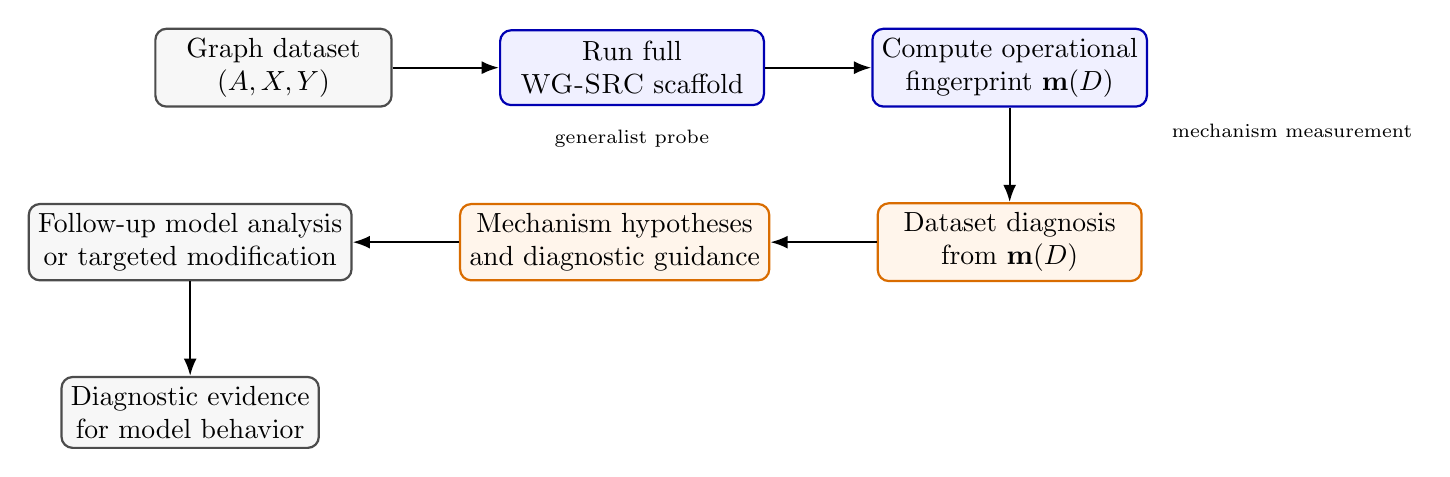
\begin{tikzpicture}[
    node distance=1.2cm and 1.35cm,
    box/.style={
        rectangle,
        rounded corners,
        draw=black!70,
        fill=gray!6,
        thick,
        align=center,
        minimum width=3.0cm,
        minimum height=0.9cm
    },
    keybox/.style={
        rectangle,
        rounded corners,
        draw=blue!70!black,
        fill=blue!6,
        thick,
        align=center,
        minimum width=3.35cm,
        minimum height=0.95cm
    },
    designbox/.style={
        rectangle,
        rounded corners,
        draw=orange!85!black,
        fill=orange!8,
        thick,
        align=center,
        minimum width=3.35cm,
        minimum height=0.95cm
    },
    arrow/.style={-{Latex[length=2.2mm]}, thick}
]

% top row
\node[box] (data) {Graph dataset\\$(A,X,Y)$};
\node[keybox, right=of data] (full) {Run full\\\textsc{WG-SRC} scaffold};
\node[keybox, right=of full] (atlas) {Compute operational\\fingerprint $\mathbf{m}(D)$};

% bottom row
\node[designbox, below=of atlas] (diagnosis) {Dataset diagnosis\\from $\mathbf{m}(D)$};
\node[designbox, left=of diagnosis] (design) {Mechanism hypotheses\\and diagnostic guidance};
\node[box, left=of design] (validate) {Follow-up model analysis\\or targeted modification};
\node[box, below=of validate] (out) {Diagnostic evidence\\for model behavior};

% arrows
\draw[arrow] (data) -- (full);
\draw[arrow] (full) -- (atlas);
\draw[arrow] (atlas) -- (diagnosis);
\draw[arrow] (diagnosis) -- (design);
\draw[arrow] (design) -- (validate);
\draw[arrow] (validate) -- (out);

% small annotations
\node[align=center, font=\scriptsize, below=0.18cm of full] {generalist probe};
\node[align=left, font=\scriptsize, below right=0.08cm and 0.18cm of atlas]
{mechanism measurement};

\end{tikzpicture}
\caption{
Mechanism atlas as a dataset diagnostic probe. \SRC{} first performs prediction
with the full scaffold and then exposes an operational fingerprint
$\mathbf{m}(D)$. The atlas is not claimed to automate model design; rather, it
produces mechanism hypotheses and post-evaluation diagnostic guidance whose support is
evaluated through aligned interventions, error shifts, and PCA--Ridge decision phase portraits on the same
measured dataset.
}
\label{fig:atlas-guided-diagnosis}
\end{figure}

\begin{table}[t]
\centering
\footnotesize
\caption{
From dataset fingerprint to post-evaluation same-dataset diagnostic guidance.
The atlas signatures generate mechanism hypotheses and diagnostic guidance for
later model analysis and dataset-specific modification on the measured dataset. The table is
a diagnostic-consistency summary, not a test-set-tuned model search: it
records whether the suggested mechanism direction agrees with aligned
interventions.
}
\label{tab:atlas-diagnostic-consistency}
\resizebox{\linewidth}{!}{%
\begin{tabular}{p{0.25\linewidth}p{0.27\linewidth}p{0.42\linewidth}}
\toprule
Atlas signature & Dataset diagnosis & Diagnostic guidance \\
\midrule
High $L_D$, low $H_D$, and positive $\Delta H_D$
& High-pass components may act as noise
& Remove, downweight, gate, or regularize high-pass blocks \\
Near-zero $R_D$ and high $C_D$
& Raw features are insufficient; class geometry is complex
& Preserve graph-derived signals and improve class-specific subspace modeling \\
High $H_D$ and negative $\Delta H_D$
& Correct nodes rely on high-pass structure
& Preserve or adaptively gate high-pass differences rather than removing them globally \\
High $Q^{\mathrm{ridge}}_D$
& Boundary decisions correct PCA failures
& Strengthen the discriminative head or improve PCA--Ridge boundary fusion \\
High $Q^{\mathrm{hard}}_D$
& Both geometry and boundary fail on many nodes
& Investigate new signal blocks, hard-node treatment, uncertainty handling, or graph rewiring \\
High $R_D$ and low-to-moderate $C_D$
& Raw features carry strong class information
& Use raw-preserving skip design, weak propagation, or propagation gating \\
\bottomrule
\end{tabular}%
}
\end{table}

This is the main inferential role of the aligned interventions. They are
deliberately simple and are not presented as the final space of improved graph
algorithms. Their purpose is to test whether atlas signatures have directional validity as
post-evaluation diagnostic guidance. When the fingerprint suggests that a mechanism is harmful
or necessary, the corresponding intervention often changes performance in the
predicted direction. For the two Amazon graphs, the atlas shows high low-pass
mass, low high-pass mass, and errors with increased high-pass signal; the
no-high-pass intervention moves in the expected direction. For Chameleon, the
atlas shows almost no raw signal, substantial high-pass structure, and high
class-subspace complexity; the raw-only variant collapses, consistent with the
diagnosis that graph-derived signals are necessary. For Texas, the large
ridge-corrected decision quadrant matches strong boundary-oriented behavior.
For Wisconsin, the high raw share matches strong raw-only behavior.

Accordingly, the claim is not that \SRC{} automatically designs new algorithms
or solves architecture search. The supported claim is that \SRC{} is a
dual-purpose white-box model: it performs prediction and produces an
operational dataset fingerprint whose mechanism hypotheses are supported by
aligned interventions and whose post-evaluation diagnostic guidance can inform
later model analysis and dataset-specific modification. In this sense, the
atlas is not merely a descriptive visualization layer; it is a diagnostic
interface between prediction, mechanism measurement, and mechanism-guided
follow-up model analysis.



\section{Limitations}
First, \SRC{} is not a universal speed improvement. The explicit audit trail
costs computation because the method constructs named graph-signal blocks,
performs Fisher selection, fits class-wise PCA subspaces, solves ridge systems,
and searches validation configurations. We therefore report the runtime table
only as an appendix computational profile rather than as a main-text speed
claim; see Appendix~\ref{app:computational-profile}. Second, the method is a
modular scaffold rather than a single irreducible architecture: specialized
variants can outperform the full scaffold on some datasets, but the atlas
should be interpreted as a diagnostic probe rather than an automatic
model-design system. Third, the baseline comparison is limited to the disclosed
reproduced suite; broader benchmarking against every recent graph learner is
future work. Fourth, the current atlas evidence is diagnostic rather than fully
causal or fully search-optimal: it is validated through aligned intervention
consistency, not through an exhaustive search over all possible redesigns.

\section{Conclusion}
We presented \SRC, a white-box graph classifier that replaces hidden message
passing with explicit graph signal blocks and replaces learned representation
layers with class PCA subspaces and closed-form ridge regression. The method
is competitive with strong graph baselines in a disclosed reproduced suite,
improving by $+1.52\pp$ on average across six datasets under the aligned
baseline rerun.

The broader contribution is that \SRC{} is dual-purpose. It is not only a
classifier, but also a measurement instrument for graph datasets. Its
mechanism atlas connects dataset-level signal fingerprints, node-level error
shifts, class-subspace geometry, and PCA--Ridge decision phases to the
behavior observed in aligned mechanistic interventions. This allows the model
to reveal whether a dataset is low-pass dominated, high-pass sensitive,
boundary driven, raw-feature sensitive, or geometrically complex.

This diagnostic role is distinct from automatic algorithm design. We do not
claim that the atlas, by itself, guarantees the globally best redesign for a
dataset or replaces a full redesign search. Instead, the supported claim is more operational: after standard evaluation on
a given dataset, the atlas provides a white-box, accuracy-preserving
fingerprint whose mechanism hypotheses and diagnostic guidance are supported by
aligned interventions on that same dataset. In this sense, \SRC{} offers a
white-box path from prediction to dataset diagnosis, and from dataset diagnosis
to mechanism-guided follow-up model analysis and dataset-specific modification.

\paragraph{Future directions.}
A natural future direction is to use the measured dataset fingerprints as a
reference frame for probing black-box graph models. By evaluating black-box
architectures and their ablated components across datasets with different
fingerprints, it may become possible to identify the empirically effective
role of specific architectural components under different measured dataset
conditions. This could support a more systematic basis for dataset-specific
model analysis and targeted optimization in future work.

\section*{Reproducibility Statement}
The package includes the LaTeX source, filtered summary tables, figures, and
CSV files used to generate the tables and atlas figures. All main-text figures
and tables use only the six evaluated datasets. Model and baseline selections
are validation-only, and paired split stability is computed by matching dataset
and repeat index. The full research repository, including algorithm
implementations, experiment scripts, and iterative development records, is
available at \href{https://github.com/xkfkh/A-White-Box-Graph-Subspace-Ridge-Classifier-with-Node-Level-Signal-Atlases}{GitHub repository}.

\section*{Broader Impact Statement}
This work aims to make graph learning more transparent.
Potential positive impacts include easier auditing of graph models and better diagnosis of when graph propagation is harmful. Potential negative impacts are similar to those of node-classification systems generally: if applied to sensitive social, financial, or biological networks without care, predictions and explanations could still be misused. The proposed atlas should be treated as a diagnostic aid, not as a guarantee of fairness or causality.

\begin{thebibliography}{99}
\bibitem[Kipf and Welling(2017)]{kipf2017gcn} Kipf, T. N. and Welling, M. Semi-supervised classification with graph convolutional networks. \emph{International Conference on Learning Representations}, 2017.
\bibitem[Hamilton et~al.(2017)]{hamilton2017graphsage}
Hamilton, W. L., Ying, Z., and Leskovec, J. Inductive representation learning on
large graphs. In \emph{Advances in Neural Information Processing Systems 30
(NeurIPS 2017)}, pp.~1024--1034, 2017.
\bibitem[Veličković et~al.(2018)]{velickovic2018gat} Veličković, P., Cucurull, G., Casanova, A., Romero, A., Liò, P., and Bengio, Y. Graph attention networks. \emph{International Conference on Learning Representations}, 2018.
\bibitem[Pei et~al.(2020)]{pei2020geomgcn} Pei, H., Wei, B., Chang, K. C.-C., Lei, Y., and Yang, B. Geom-GCN: Geometric graph convolutional networks. \emph{International Conference on Learning Representations}, 2020.
\bibitem[Zhu et~al.(2020)]{zhu2020beyond} Zhu, J., Yan, Y., Zhao, L., Heimann, M., Akoglu, L., and Koutra, D. Beyond homophily in graph neural networks: Current limitations and effective designs. \emph{Advances in Neural Information Processing Systems}, 2020.
\bibitem[Lim et~al.(2021)]{lim2021linkx} Lim, D., Hohne, F., Li, X., Huang, S. L., Gupta, V., Bhalerao, O., and Lim, S.-N. Large scale learning on non-homophilous graphs: New benchmarks and strong simple methods. \emph{Advances in Neural Information Processing Systems}, 2021.
\bibitem[Chien et~al.(2021)]{chien2021gprgnn} Chien, E., Peng, J., Li, P., and Milenkovic, O. Adaptive universal generalized PageRank graph neural network. \emph{International Conference on Learning Representations}, 2021.
\bibitem[Yu et~al.(2020)]{yu2020mcr2} Yu, Y., Chan, K. H. R., You, C., Song, C., and Ma, Y. Learning diverse and discriminative representations via the principle of maximal coding rate reduction. \emph{Advances in Neural Information Processing Systems}, 2020.
\bibitem[Chan et~al.(2022)]{chan2022redunet} Chan, K. H. R., Yu, Y., You, C., Qi, H., Wright, J., and Ma, Y. ReduNet: A white-box deep network from the principle of maximizing rate reduction. \emph{Journal of Machine Learning Research}, 23(114):1--103, 2022.
\bibitem[Wang et~al.(2024)]{wang2024mcr2landscape} Wang, P., Liu, H., Pai, D., Yu, Y., Zhu, Z., Qu, Q., and Ma, Y. A global geometric analysis of maximal coding rate reduction. \emph{International Conference on Machine Learning}, 2024.
\bibitem[Pearson(1901)]{pearson1901pca} Pearson, K. On lines and planes of closest fit to systems of points in space. \emph{Philosophical Magazine}, 2(11):559--572, 1901.
\bibitem[Hoerl and Kennard(1970)]{hoerl1970ridge} Hoerl, A. E. and Kennard, R. W. Ridge regression: Biased estimation for nonorthogonal problems. \emph{Technometrics}, 12(1):55--67, 1970.
\bibitem[von Luxburg(2007)]{vonluxburg2007tutorial} von Luxburg, U. A tutorial on spectral clustering. \emph{Statistics and Computing}, 17(4):395--416, 2007.
\bibitem[Shchur et~al.(2018)]{shchur2018pitfalls} Shchur, O., Mumme, M., Bojchevski, A., and Günnemann, S. Pitfalls of graph neural network evaluation. \emph{Relational Representation Learning Workshop, NeurIPS}, 2018.
\end{thebibliography}

\appendix



\section{Computational Profile}
\label{app:computational-profile}

Table~\ref{tab:efficiency} reports a computational profile for completeness.
It is not used as a main-text speed claim. Baseline runtime and accuracy are
taken from the aligned CPU baseline rerun; \SRC{} accuracy is standardized to
the ten-repeat main-table value. The purpose of this table is to document the
cost of the white-box audit trail: explicit graph-signal construction, Fisher
selection, class-wise PCA fitting, ridge solves, and validation search.

\begin{table}[t]
\centering
\small
\caption{
Appendix computational profile. Baseline runtime and accuracy are taken from
the aligned CPU baseline rerun; \SRC{} accuracy is standardized to the
ten-repeat main-table value. This table documents runtime cost and is not
intended as a speedup claim.
}
\label{tab:efficiency}
\begin{tabular}{llrrrr}
\toprule
Dataset & Best baseline & Baseline time & \SRC{} time & Ratio & \SRC{} acc. \\
\midrule
Amazon-Computers & GraphSAGE & 208.5 & 292.9 & 1.4$\times$ & 78.71 \\
Amazon-Photo & GraphSAGE & 81.3 & 136.4 & 1.7$\times$ & 88.76 \\
Chameleon & LINKX & 3.6 & 62.1 & 17.5$\times$ & 72.48 \\
Cornell & GraphSAGE & 0.8 & 4.5 & 5.7$\times$ & 75.41 \\
Texas & GraphSAGE & 0.8 & 4.1 & 5.2$\times$ & 86.32 \\
Wisconsin & GraphSAGE & 0.9 & 6.0 & 6.8$\times$ & 84.31 \\
\bottomrule
\end{tabular}
\end{table}


\section{Implementation Details}
The Fisher feature count was selected from $K\in\{4000,5000,6000,8000\}$. The PCA maximum dimension was selected from $r_{max}\in\{32,48,64,96\}$, with energy threshold $\eta\in\{0.90,0.95,0.99\}$. Ridge regularizer sets were selected from $\{0.01,0.1,1.0\}$, $\{0.05,0.5,5.0\}$, and $\{0.1,1.0,10.0\}$. The fusion weight was selected from $w\in\{0.2,0.3,0.4,0.5,0.6,0.7,0.8\}$. All selections were made using validation accuracy. The corresponding
implementation and experiment scripts are released in the public repository
listed in the Reproducibility Statement.

\section{Class-Pair Geometry and Confusion}
\begin{figure}[H]
    \centering
    
\includegraphics[width=0.82\linewidth]{fig_chameleon_subspace_confusion.pdf}
    \caption{Chameleon class-pair geometry and confusion constellation. The left panel shows pairwise PCA subspace overlap; the right panel shows bidirectional confusion. This appendix figure illustrates how the same subspace objects used for prediction can also diagnose class-pair errors.}
    \label{fig:subspace-confusion}
\end{figure}

\end{document}
